\section{Knots as processes}\label{sec:knots_as_processes} % (fold)

This section bootstraps intuitions about the target calculus by
introducing process expressions for key aspects of a knot's
structure. An $n$ crossing knot $K$ is modeled as a system
$\meaningof{K}$ of concurrently executing processes. More
specifically, $\meaningof{K}$ is a \emph{parallel composition} $\Pi_{i
  = 0}^{n-1} \meaningof{C(i)} | W$ of $n+1$ processes consisting of
$n$ crossing processes $\meaningof{C(i)}$ and a process $W$
constituting a ``wiring harness.'' The latter process can be thought
of as the computational equivalent to Conway's ``basic polygon,'' if
the knot is in minimal crossing number form. The complete expression
of the encoding is

% \begin{eqnarray*}
%   \meaningof{K} & := &  (v_0 ... v_{4n-1})( \Pi_{i = 0}^{n-1} (\nu \; u)\meaningof{C(i)}(v_{4i},...,v_{4i+3},u) \\
%   & & \; \; \; \; \; \; \; \; \; \; \; \; \; \; \; \; \; \; | \Pi_{i = 0}^{n-1} W(v_{\omega(i,0)},v_{\omega(i,1)})|W(v_{\omega(i,2)},v_{\omega(i,3)}) ) \nonumber
% \end{eqnarray*}

\begin{align*}
  \meaningof{K} :=  (v_0 ... v_{4n-1}) & ( \Pi_{i = 0}^{n-1} (\nu \; u)\meaningof{C(i)}(v_{4i},...,v_{4i+3},u) \\
  & | \Pi_{i = 0}^{n-1} W(v_{\omega(i,0)},v_{\omega(i,1)})|W(v_{\omega(i,2)},v_{\omega(i,3)}) )
\end{align*}

Here, $C(i)$ represents the $i$th crossing in the knot diagram $K$.  The wiring process, $\Pi_{i =
  0}^{n-1}W(v_{\omega(i,0)},v_{\omega(i,1)})|W(v_{\omega(i,2)},v_{\omega(i,3)})$,
is itself a parallel composition of wire processes that correspond to
edges in the 4-valent graph of the knot shadow \cite{SchareinPhD} the constraints of
which are reflected in the indexing function $\omega$. The wiring process
may be calculated from other knot notations. For example,  we later show how the indexing function $\omega$ may be calculated
from $\delta$, the DT code of the knot projection. The crossing and wire
processes have further substructure, outlined below.

\begin{remark}[knots as abstractions]
  The reader familiar with process calculi will observe that the
  encoding actually produces an \emph{abstraction} \cite{SangiorgiWalker}  in $4\#(K)$ names
  (see the first choice in the production labeled agent in the grammar
  of \ref{sub:the_syntax_and_semantics_of_the_notation_system}). This is actually a way of demarking that the encoding should
  be insensitive to the particular set of names chosen to represent the
  ports of the crossings. Some caution must be exercised, however, as
  the encoding only preserves knot structure if the abstraction is
  applied to a vector of $4\#(K)$ distinct names.
\end{remark}

\subsection{Crossing processes}\label{sub:crossing_processes} % (fold)
A crossing is conceived in the diagram below as a black-box having
four points of external interaction (\emph{ports}) with the remainder
of the knot process and as having two internal wires each connecting a
pair of ports. As a process, the crossing has four possible behaviors,
as shown in the defining encoding below.
\begin{figure}[hbp]
    \centering
    \scalebox{0.27}[0.270]{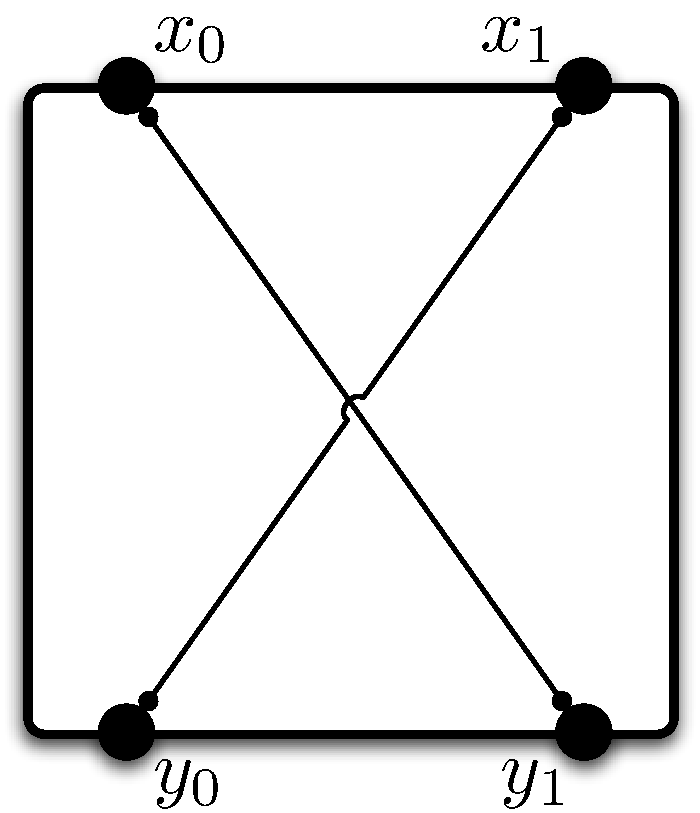
\includegraphics[viewport=0 0 390 360]{../../illustrations/BasicCrossingCircuit.pdf}}
    \caption{ Crossing process }
\end{figure}
\begin{eqnarray*}
   C(x_0,x_1,y_0,y_1,u) & \plogp   & x_1?(s).y_0!(s).(C(x_0,x_1,y_0,y_1,u)|u!) \nonumber \\
  & & + y_0?(s).x_1!(s).(C(x_0,x_1,y_0,y_1,u)|u!) \nonumber \\
  & & + x_0?(s).u?.y_1!(s).(C(x_0,x_1,y_0,y_1,u)) \nonumber \\
  & & + y_1?(s).u?.x_0!(s).(C(x_0,x_1,y_0,y_1,u)) \nonumber
\end{eqnarray*}

A crossing process has four ports $x_0,x_1,y_0,y_1$ and a hidden
synchronizer $u$. Each port has a partner port, linked as shown in the
diagram (note the relationship to Conway's $\pm 1$ tangles
\cite{Conway1970An-enumeration-}). For example, the first behavior (indicated by the first
term of the summand) is that the process listens at port $x_1$ for a
signal $s$ (which will come, if at all, via the wiring
process). Having heard $s$, the signal is passed directly to the port
$y_0$ where the signal is then broadcast via the wiring process. Then
the process alerts the hidden synchronizer $u$ that a signal has been
passed between the ports, while concurrently preparing itself for
further signal processing. The second summand represents a signal
passing along the same strand in the opposite direction. The third and
fourth summands are similar to the first two, except that before
passing any received signal to its partner port, the process waits for
a signal from the synchronizer $u$ before allowing the signal to
pass. So the role of $u$ is that of a traffic controller who gives
priority to traffic over the route between $x_1$ and $y_0$, mimicking
an over-crossing.

\subsection{Wirings}\label{sub:wirings} % (fold)

As an illustration of the expressive power of the formalism, taken
together with the short description of the process calculus in the next
section, the definitions below fully equip the interested reader to
verify that wire processes are lossless, infinite capacity buffers. 


\begin{eqnarray*}
    W(x,y) & \plogp & (\nu \; n \; m)(Waiting(x,n,m) | Waiting(y,m,n)) \nonumber \\
Waiting(x,c,n) & \plogp   & x?(v).(\nu \; m)(Cell(n,v,m) | Waiting(x,c,m)) \nonumber \\
  & & + c?(w).c?(c).Ready(x,c,n,w) \nonumber \\
  Ready(x,c,n,w) & \plogp  & x?(v).(\nu \; m)(Cell(n,v,m) | Ready(x,c,m,w)) \nonumber \\
  & & + x!(w).Waiting(x,c,n) \nonumber \\
  Cell(c,v,n) & \plogp & c!(v).c!(n).0 \nonumber
\end{eqnarray*}

The ports $x$ and $y$ in which $W$ is \emph{parameterized} may be
intuitively considered splice points in the knot diagram. We adopt
this terminology in the sequel.

One may well wonder why perfect buffers are chosen to represent
wires. For example, the following process intuitively captures a notion of wire.

\begin{equation*}
  Relay(x,y) := x?(s).y!(s).Relay(x,y) + y?(s).x!(s).Relay(x,y)
\end{equation*}

The problem is one of composition. Foreshadowing the method of proof,
in the sequel we will need to compose wires and crossings and have the
result act as a wire. For example, if $W(x,y)$ represents a candidate
for wire behavior, to model the first Reidemeister move we have a demand that

\begin{equation*}
  W(y_{0},y_{1}) \simeq (\nu \; x_{0} \; x_{1} \; w_{0} \; w_{1} )(W(y_{0},w_{0}) |(\nu \; u)C(x_{0},x_{1},w_{0},w_{1},u) | W(x_{0},x_{1}) | W(y_{1},w_{1}))
\end{equation*}

Again, the reader may verify that while this is true of buffers, it is
not true of the $Relay$ process defined above.
